\begin{exercice}
    Écrire l'abscisse de chaque point.
    \begin{enumerate}
        \item \raisebox{-0.5\totalheight}[0.5\totalheight]{\raisebox{\depth}{
        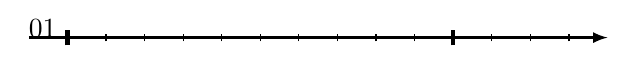
\begin{tikzpicture}[scale=0.49]            
            % Axe
            \draw[thick,>=latex,->](0,0)--+(15,0);
            \foreach \x in {1,...,14} \draw (\x,-.1) -- (\x,0.1);
            \coordinate (O) at (1,0);
            \coordinate (I) at (11,0);
            \draw[ultra thick] (1,-.2) -- (1,0.2);
            \draw[ultra thick] (11,-.2) -- (11,0.2);
            \tkzLabelPoint[below,yshift=-3](O){$0$};
            \tkzLabelPoint[below,yshift=-3](I){$1$};
            % Points supplémentaires
            \coordinate (A) at (4,0);
            \coordinate (B) at (9,0);
            \coordinate (C) at (12,0);
            \coordinate (D) at (14,0);
            \tkzDrawPoints[shape=cross out,size=3pt](A,B,C,D);
            \tkzLabelPoints[above](A,B,C,D);
        \end{tikzpicture}
        }}
        \item \raisebox{-0.5\totalheight}[0.5\totalheight]{\raisebox{\depth}{
        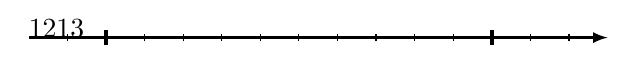
\begin{tikzpicture}[scale=0.49]            
            % Axe
            \draw[thick,>=latex,->](0,0)--+(15,0);
            \foreach \x in {1,...,14} \draw (\x,-.1) -- (\x,0.1);
            \coordinate (O) at (2,0);
            \coordinate (I) at (12,0);
            \draw[ultra thick] (2,-.2) -- (2,0.2);
            \draw[ultra thick] (12,-.2) -- (12,0.2);
            \tkzLabelPoint[below,yshift=-3](O){$12$};
            \tkzLabelPoint[below,yshift=-3](I){$13$};
            % Points supplémentaires
            \coordinate (E) at (3,0);
            \coordinate (F) at (5,0);
            \coordinate (G) at (7,0);
            \coordinate (H) at (13,0);
            \tkzDrawPoints[shape=cross out,size=3pt](E,F,G,H);
            \tkzLabelPoints[above](E,F,G,H);
        \end{tikzpicture}
        }}
        \item \raisebox{-0.5\totalheight}[0.5\totalheight]{\raisebox{\depth}{
        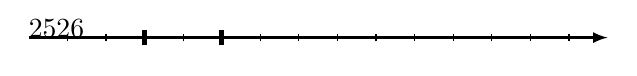
\begin{tikzpicture}[scale=0.49]            
            % Axe
            \draw[thick,>=latex,->](0,0)--+(15,0);
            \foreach \x in {1,...,14} \draw (\x,-.1) -- (\x,0.1);
            \coordinate (O) at (3,0);
            \coordinate (I) at (5,0);
            \draw[ultra thick] (3,-.2) -- (3,0.2);
            \draw[ultra thick] (5,-.2) -- (5,0.2);
            \tkzLabelPoint[below,yshift=-3](O){$25$};
            \tkzLabelPoint[below,yshift=-3](I){$26$};
            % Points supplémentaires
            \coordinate (J) at (4,0);
            \coordinate (K) at (8,0);
            \coordinate (L) at (12,0);            
            \tkzDrawPoints[shape=cross out,size=3pt](J,K,L);
            \tkzLabelPoints[above](J,K,L);
        \end{tikzpicture}
        }}
        \item \raisebox{-0.5\totalheight}[0.5\totalheight]{\raisebox{\depth}{
            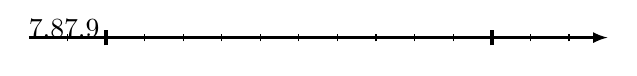
\begin{tikzpicture}[scale=0.49]            
                % Axe
                \draw[thick,>=latex,->](0,0)--+(15,0);
                \foreach \x in {1,...,14} \draw (\x,-.1) -- (\x,0.1);
                \coordinate (O) at (2,0);
                \coordinate (I) at (12,0);
                \draw[ultra thick] (2,-.2) -- (2,0.2);
                \draw[ultra thick] (12,-.2) -- (12,0.2);
                \tkzLabelPoint[below,yshift=-3](O){$\num{7.8}$};
                \tkzLabelPoint[below,yshift=-3](I){$\num{7.9}$};
                % Points supplémentaires
                \coordinate (M) at (3,0);
                \coordinate (N) at (5,0);
                \coordinate (P) at (11,0);
                \coordinate (Q) at (13,0);
                \tkzDrawPoints[shape=cross out,size=3pt](M,N,P,Q);
                \tkzLabelPoints[above](M,N,P,Q);
            \end{tikzpicture}
            }}            
            \item \raisebox{-0.5\totalheight}[0.5\totalheight]{\raisebox{\depth}{
                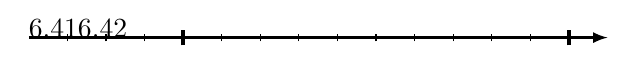
\begin{tikzpicture}[scale=0.49]            
                    % Axe
                    \draw[thick,>=latex,->](0,0)--+(15,0);
                    \foreach \x in {1,...,14} \draw (\x,-.1) -- (\x,0.1);
                    \coordinate (O) at (4,0);
                    \coordinate (I) at (14,0);
                    \draw[ultra thick] (4,-.2) -- (4,0.2);
                    \draw[ultra thick] (14,-.2) -- (14,0.2);
                    \tkzLabelPoint[below,yshift=-3](O){$\num{6.41}$};
                    \tkzLabelPoint[below,yshift=-3](I){$\num{6.42}$};
                    % Points supplémentaires
                    \coordinate (V) at (2,0);
                    \coordinate (W) at (7,0);
                    \coordinate (Y) at (10,0);
                    \coordinate (Z) at (12,0);
                    \tkzDrawPoints[shape=cross out,size=3pt](V,W,Y,Z);
                    \tkzLabelPoints[above](V,W,Y,Z);
                \end{tikzpicture}
                }}
    \end{enumerate}
 \end{exercice}
 
 \begin{corrige}
   \ \\ [-5mm]
   \begin{enumerate}
      \item $A({\blue 0,3}) \; ; \; B({\blue 0,8}) \; ; \; C({\blue 1,1}) \; ; \; D({\blue 1,3})$.
      \item $E({\blue 12,1}) \; ; \; F({\blue 12,3}) \; ; \; G({\blue 12,5}) \; ; \; H({\blue 13,1})$.
      \item $J({\blue 25,5}) \; ; \; K({\blue 27,5}) \; ; \; L({\blue 29,5})$.
      \item $M({\blue 7,81}) \; ; \; N({\blue 7,83}) \; ; \; P({\blue 7,89}) \; ; \; Q({\blue 7,91})$.
      \item $V({\blue 6,408}) \; ; \; W({\blue 6,413}) \; ; \; Y({\blue 6,416}) \; ; \; Z({\blue 6,418})$.
   \end{enumerate}
 \end{corrige}
